\section{Test}
The aim of the project is to create a good base on which multiplayer games can easily be created. It is therefore desirable that the server is stable and able to handle a decent number of games at the same time without significant response time. More specifically we want a single server to be able to host as many games as possible without surpassing an average response time of 1000ms. Additionally we want to locate possible bottlenecks in the code, by recording the run time of each API call. This can be tested using a black-box testing.

The Python scripts used to test the server can be found in the folder named Test with the rest of the source code.\fixme{ret i forhold til hvor det ligger}

\subsection{Test Setup}
\label{sec:testSetup}
The test is done by simulating users through Python scripts: One for simulating a number of active games with the purpose of creating some artificial server load, and one for making single API calls and collecting data.

The first script creates server load by spawning a thread per desired game. Each thread creates a game, makes relevant API calls for the duration of the test, and finally it deletes the game. Each thread simulates very busy games with 2 API calls per second. 

The other script makes a single API call a number\fxfatal{what number?} of times, collects the run time for each call and finally calculates the mean and standard deviation. Because the goal is to stay on a run time under 1000ms, the number of calls taking more than this is also recorded.

Each script is run on seperate computers, to be sure the extra processing power needed to handle the game threats does not influence the test results. 

%The following API calls are used in the test:
%\begin{itemize}
%\item Login
%\item Create game
%\item Delete game
%\item Join game
%\item Leave game
%\item Change location
%\item Invite player
%\item List public games
%\item List joined games
%\item Get game info
%\item Shoot
%\end{itemize}

\subsection{Test Results}
<Results and things we learned from the tests.>
%In table \cref{tab:testRes} the results from the test are shown\fixme{Just latency test?}. Each test was perfomed with half a second interval.

\begin{figure}[H]
  \centering
  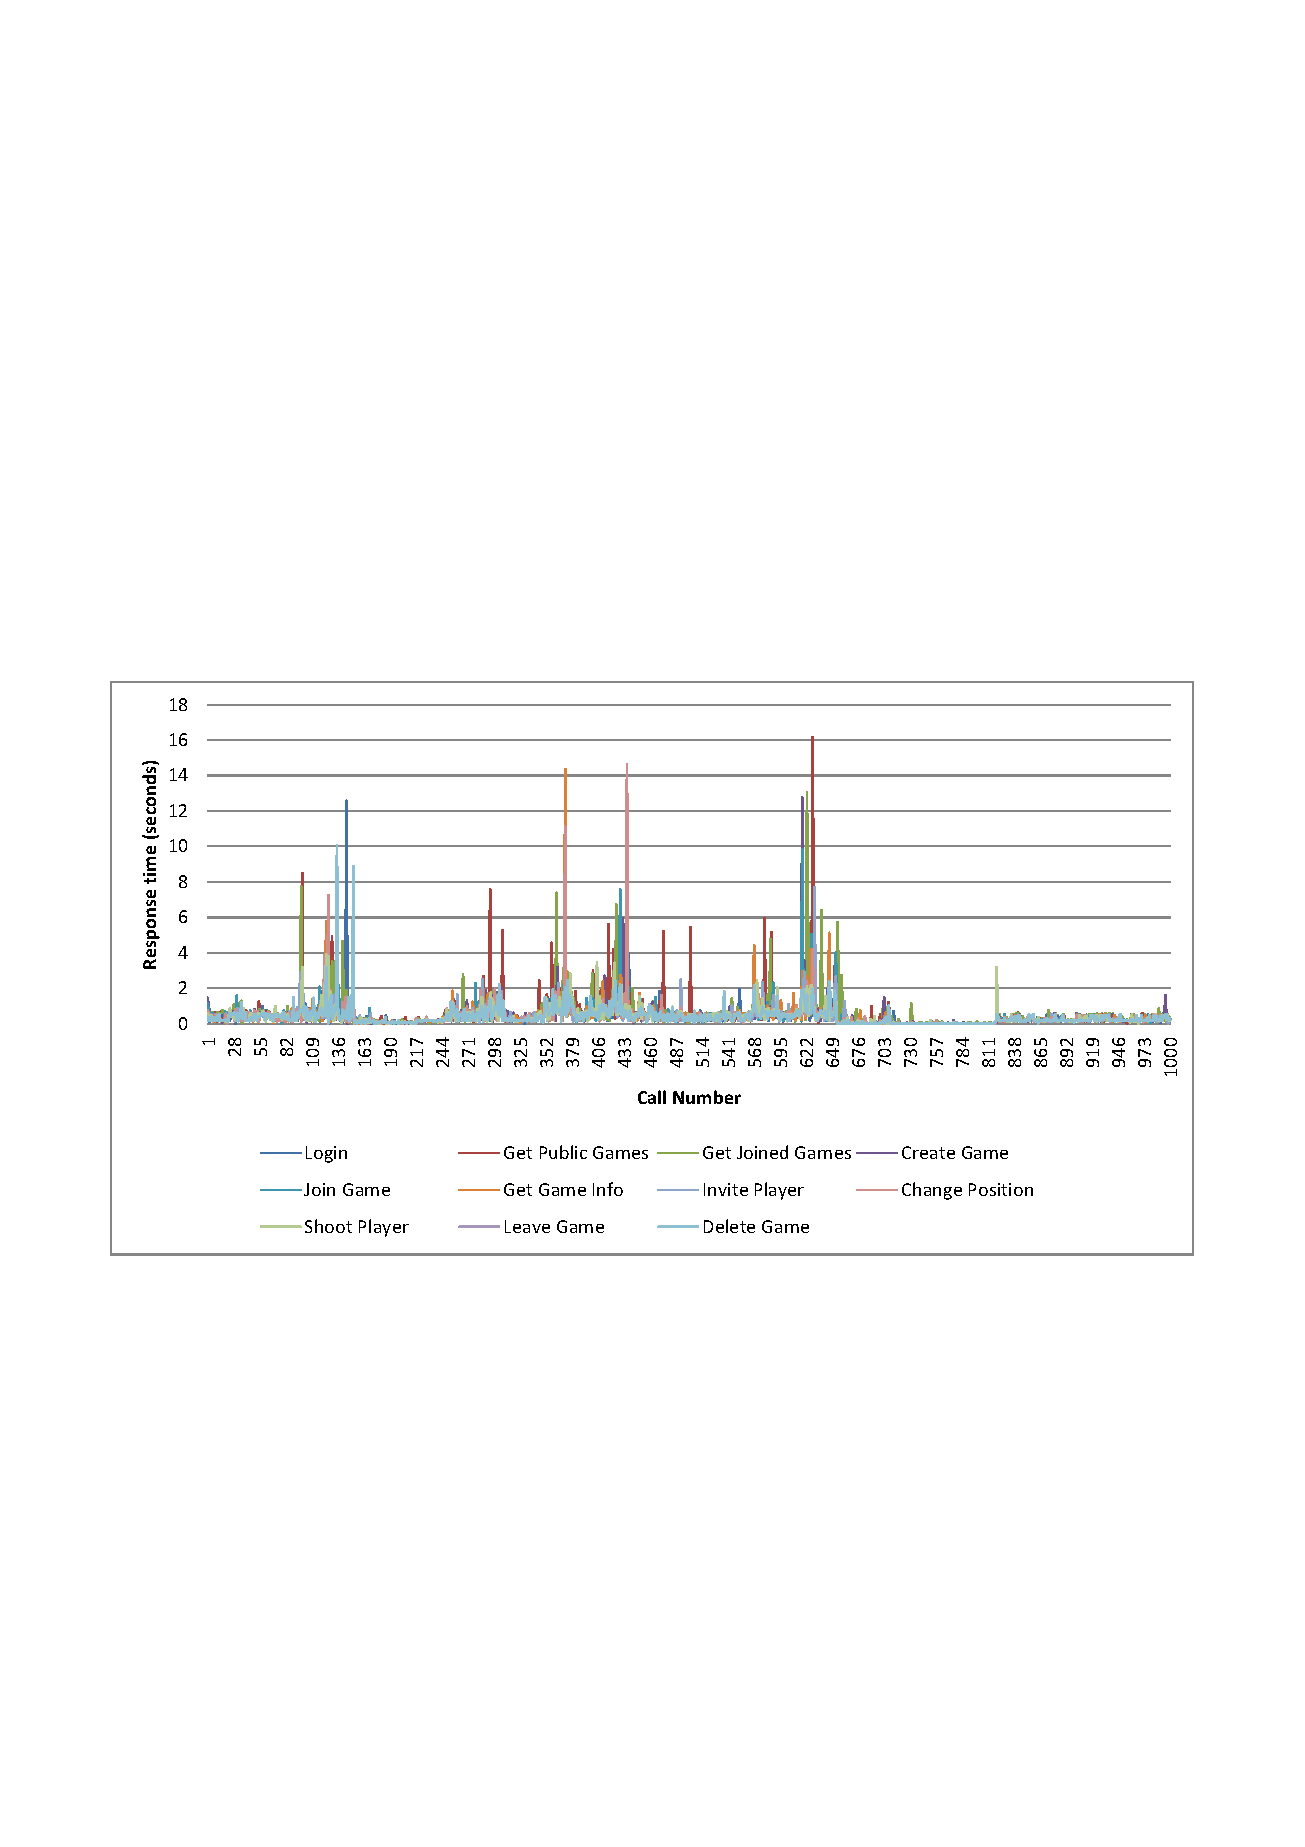
\includegraphics[width=\textwidth, clip=true, trim=0 22em 0 22em]{billeder/loadgraph.pdf}  
  \caption{Graph showing the response time of each API call.}
  \label{fig:loadgraph}
\end{figure}

\renewcommand{\arraystretch}{1.2}
\begin{table}
\label{tab:1}
\caption{Test}
\centering
\begin{tabular}{|l|>{\raggedleft\arraybackslash}p{5em}|>{\raggedleft\arraybackslash}p{5em}|>{\raggedleft\arraybackslash}p{5em}|>{\raggedleft\arraybackslash}p{5em}|}
	\hline  & \multicolumn{1}{p{5em}|}{Mean} & \multicolumn{1}{p{5em}|}{Standard deviation} & \multicolumn{1}{p{5em}|}{\# over limit} \\ 
	\hline Login  &  &  &  \\ 
	\hline Get public games  &  &  &  \\ 
	\hline Get joined games  &  &  &  \\ 
	\hline Create game  &   &  &  \\ 
	\hline Delete game  &  &  &  \\ 
	\hline Join game  &  &  &  \\ 
	\hline Leave game  &  &  &  \\ 
	\hline Game info  &  &  &  \\ 
	\hline Invite player  &  &  &  \\ 
	\hline Change position  &  &  &  \\ 
	\hline Shoot  &  &  &  \\ 
	\hline 
\end{tabular} 
\end{table}

\begin{table}
\label{tab:2}
\caption{Test}
\centering
\begin{tabular}{|l|>{\raggedleft\arraybackslash}p{5em}|>{\raggedleft\arraybackslash}p{5em}|>{\raggedleft\arraybackslash}p{5em}|>{\raggedleft\arraybackslash}p{5em}|}
	\hline  & \multicolumn{1}{p{5em}|}{Mean} & \multicolumn{1}{p{5em}|}{Standard deviation} & \multicolumn{1}{p{5em}|}{\# over limit} \\ 
	\hline Login  &  &  &  \\ 
	\hline Get public games  &  &  &  \\ 
	\hline Get joined games  &  &  &  \\ 
	\hline Create game  &   &  &  \\ 
	\hline Delete game  &  &  &  \\ 
	\hline Join game  &  &  &  \\ 
	\hline Leave game  &  &  &  \\ 
	\hline Game info  &  &  &  \\ 
	\hline Invite player  &  &  &  \\ 
	\hline Change position  &  &  &  \\ 
	\hline Shoot  &  &  &  \\ 
	\hline 
\end{tabular} 
\end{table}
\renewcommand{\arraystretch}{1}












%\subsubsection{Test}
%\subsubsection{Login}
%\subsubsection{Game creation}
%\subsubsection{Join game}
%\subsubsection{Leave game}
%\subsubsection{Update player location}
%\subsubsection{Edit player invites}
%\subsubsection{Invite player}
%\subsubsection{title}




%\subsection{Sources of Error}
%There are a number of factors that possibly affect to the accuracy of the tests.\\

%One of the main sources of error is found in the nature\fixme{Overkill at sige nature?} of the internet. The tests were performed on a small local network and connections were sometimes closed because there was a fallout in the network. The test script, which the spammer, described in \cref{sec:testSetup}, then reconnected as soon as possible to maintain the highest possible amount of stress on the victim server. 